\documentclass[a4paper,12pt]{article}
\usepackage[a4paper,margin=1in]{geometry}
\usepackage{graphicx}
\usepackage{titlesec}
\usepackage{setspace}
\usepackage{fancyhdr}
\usepackage{fontspec}
\usepackage{color}
\usepackage{tikz}
\usetikzlibrary{arrows.meta}
\usepackage{circuitikz}
\usepackage{float}
\usepackage{amsmath}
\usepackage{longtable}
\usepackage{multirow}
\usepackage{array}
\pagestyle{empty}
\begin{document}

\begin{titlepage}
    \centering
    \vspace*{1cm}
    
    {\scshape\LARGE Indian Institute of Technology Hyderabad \par}
    \vspace{0.5cm}
    {\scshape\Large Department of Electrical Engineering \par}
    \vspace{1.5cm}
    
    \rule{\linewidth}{0.5mm} \\[0.4cm]
    { \huge \bfseries Experiment 9: Sequence Detector \\[0.3cm]
      \Large (Moore Machine Implementation using Flip-Flops and Logic Gates) }\\[0.4cm]
    \rule{\linewidth}{0.5mm} \\[2cm]
    
    \begin{minipage}{0.45\textwidth}
        \begin{flushleft} \large
        \textbf{Submitted By:}\\
        Krishna Hanumanth Patil \\
        Roll No: EE24BTECH11036 \\
        Deepak Kumar Ahirwar \\
        Roll No: EE24BTECH11014 \\
        \end{flushleft}
    \end{minipage}%
    \hfill
    \begin{minipage}{0.45\textwidth}
        \begin{flushright} \large
        \textbf{Submitted To:} \\
        Prof. Gajendranath Chaudhury \\
        Department of Electrical Engineering \\
        \end{flushright}
    \end{minipage}\\[2cm]
    
    \begin{center}
        \textbf{Course Code:} EE1501\\
        \textbf{Course Name:} Electric Circuits Laboratory \\
        \vfill
        {\large \today\par}
    \end{center}
\end{titlepage}

\newpage
\tableofcontents
\newpage

\section{What is a Finite State Machine}

A Finite State Machine (FSM) is a mathematical model of computation used to represent the behavior of sequential systems. It operates in one of a finite number of states at any given time and transitions between states in response to external inputs. The machine's next state and output are determined by its current state and input, governed by well-defined transition and output functions. \\

The FSM is characterized by:

\begin{itemize}
    \item \textbf{External Inputs:} Signals received from outside the system, used to determine transitions.
    \item \textbf{Externally Visible Outputs:} Signals generated based on the internal state and/or inputs.
    \item \textbf{Internal State:} Stored information that represents the current status of the system, typically maintained using flip-flops.
\end{itemize}

The FSM transitions between a finite number of internal states in response to clocked inputs, producing outputs according to its defined behavior.

\section{Finite State Machines: Moore and Mealy Models}

The finite state machine (FSM) can be classified into two main types based on how the outputs are generated: the \textbf{Moore Model} and the \textbf{Mealy Model}. These two models define the relationship between the current state, inputs, and outputs in different ways, affecting how the system's behavior is observed.

In an FSM, the behavior is typically classified as either \textbf{Moore} or \textbf{Mealy}, depending on how outputs are derived.

\subsection{Moore Model}

In the \textbf{Moore Model}, the \textbf{outputs} depend solely on the \textbf{current state} of the machine. The output remains constant for each state and only changes when the system transitions to a new state.

\subsubsection{Key Features of the Moore Model:}
\begin{itemize}
    \item Outputs depend only on the current state.
    \item The output changes only when the system enters a new state.
    \item Simpler to design because the output is directly linked to the state, and no input is involved in determining the output.
\end{itemize}

\subsection*{Mealy Model}

In the \textbf{Mealy Model}, the \textbf{outputs} depend on both the \textbf{current state} and the \textbf{inputs}. This allows the output to change immediately when the input changes, even without a state transition.

\subsubsection*{Key Features of the Mealy Model:}
\begin{itemize}
    \item Outputs depend on both the current state and the inputs.
    \item The output can change immediately with the input, without needing a state transition.
    \item More compact and efficient since outputs can change based on inputs without transitioning to a new state.
\end{itemize}

For this experiment, we are using the \textbf{MOORE MODEL} to detect a sequence, namely \textbf{11011} ; in fact we will try to detect it overlappingly and repeatedly .

\section{Hardware Requirements for Moore Model Sequence Detector}
\begin{itemize}
	\item 3 J-K flip flops (2 IC 74LS76N) (T flip flops would be even better)
	\item 10 and gates or 4 3-input and gate ic (IC 74LS11N)
	\item 6 or gates or 3 2-input or gate ic (IC 74LS32N)
	\item one nand gate (IC 74HC00N)
	\item an led or any thing that can be used to show that the sequence is detected
        \item Jumper wires 
	\item Breadboards 
\end{itemize}

\newpage

\section{State Diagram}

Below shown diagram represents the required FSM that as to be implemented for our experiment .
\begin{figure}[H]
    \centering
    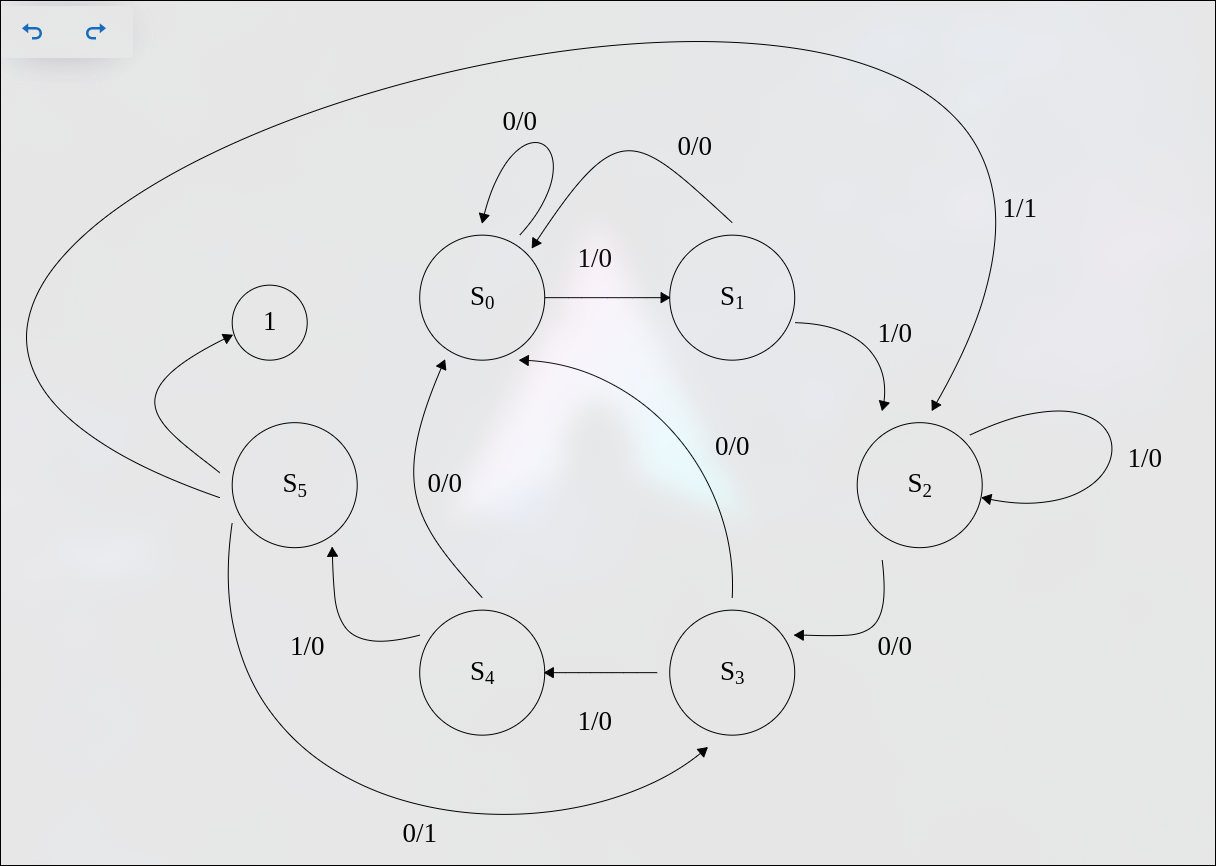
\includegraphics[width=0.8\textwidth]{figs/state.png}
    \caption{State Diagram}
    \label{fig:your_image_label}
\end{figure}

As shown in the diagram, the sequence detector can be represented as a set of different states, we use it to get a state transition table which is discussed in the next section .

\section{State Transition Table}
\begin{longtable}{|c|c|c|c||c|c|c||c|c|c|c|}
\caption{State Transition Table with Q(t) and Q(t+1) Group Labels} \\
\hline
\multicolumn{4}{|c||}{} & \multicolumn{3}{c||}{Q(t)} & \multicolumn{4}{c|}{Q(t+1)} \\
\multicolumn{4}{|c||}{Q(t)} & \multicolumn{3}{c||}{T Flip-Flop Inputs} & \multicolumn{3}{c|}{State} & \multirow{2}{*}{Y} \\
Q\textsubscript{2} & Q\textsubscript{1} & Q\textsubscript{0} & X & T\textsubscript{2} & T\textsubscript{1} & T\textsubscript{0} & Q\textsubscript{2} & Q\textsubscript{1} & Q\textsubscript{0} & \\
\hline
\endfirsthead

\hline
\multicolumn{4}{|c||}{} & \multicolumn{3}{c||}{Q(t)} & \multicolumn{4}{c|}{Q(t+1)} \\
\multicolumn{4}{|c||}{Q(t)} & \multicolumn{3}{c||}{T Flip-Flop Inputs} & \multicolumn{3}{c|}{State} & \multirow{2}{*}{Y} \\
Q\textsubscript{2} & Q\textsubscript{1} & Q\textsubscript{0} & X & T\textsubscript{2} & T\textsubscript{1} & T\textsubscript{0} & Q\textsubscript{2} & Q\textsubscript{1} & Q\textsubscript{0} & \\
\hline
\endhead

\hline
\endfoot

\hline
\endlastfoot

0 & 0 & 0 & 0 & 0 & 0 & 0 & 0 & 0 & 0 & 0 \\
0 & 0 & 0 & 1 & 0 & 0 & 1 & 0 & 0 & 1 & 0 \\
\hline
0 & 0 & 1 & 0 & 0 & 0 & 1 & 0 & 0 & 0 & 0 \\
0 & 0 & 1 & 1 & 0 & 1 & 1 & 0 & 1 & 0 & 0 \\
\hline
0 & 1 & 0 & 0 & 0 & 0 & 1 & 0 & 1 & 1 & 0 \\
0 & 1 & 0 & 1 & 0 & 0 & 0 & 0 & 1 & 0 & 0 \\
\hline
0 & 1 & 1 & 0 & 0 & 1 & 1 & 0 & 0 & 0 & 0 \\
0 & 1 & 1 & 1 & 1 & 1 & 1 & 1 & 0 & 0 & 0 \\
\hline
1 & 0 & 0 & 0 & 1 & 0 & 0 & 0 & 0 & 0 & 0 \\
1 & 0 & 0 & 1 & 0 & 0 & 1 & 1 & 0 & 1 & 0 \\
\hline
1 & 0 & 1 & 0 & 1 & 1 & 0 & 0 & 1 & 1 & 1 \\
1 & 0 & 1 & 1 & 1 & 1 & 1 & 0 & 1 & 0 & 1 \\
\hline
1 & 1 & 0 & 0 & X & X & X & X & X & X & X \\
1 & 1 & 0 & 1 & X & X & X & X & X & X & X \\
\hline
1 & 1 & 1 & 0 & X & X & X & X & X & X & X \\
1 & 1 & 1 & 1 & X & X & X & X & X & X & X \\
\end{longtable}

This is the state transition table , using this we determine the SOP form of the boolean functions for $T_0,T_1,T_2,y$ so that the state machine be implemented using T flip flops and obviously some logic gates.This can be easily done using K-maps.

\section{Determining the boolean functions}

Let's, start with the K-map for $Q_0$,
\[
\begin{array}{|c|c|c|c|c|}
\hline
Q_2 Q_1 \backslash Q_0 x & 00 & 01 & 11 & 10 \\
\hline
00 & 0 & 1 & 1 & 1 \\
\hline
01 & 1 & 0 & 1 & 1 \\
\hline
11 & X & X & X & X \\
\hline
10 & 0 & 1 & 1 & 0 \\
\hline
\end{array}
\]

Now , after simplifying, we get
\[
\boxed{T_0 = \overline{Q_2}Q_0 + Q_1 \overline{x} + \overline{Q_1}x} 
\]

Next, for $Q_1$,
\[
\begin{array}{|c|c|c|c|c|}
\hline
Q_2 Q_1 \backslash Q_0 x & 00 & 01 & 11 & 10 \\
\hline
00 & 0 & 0 & 1 & 0 \\
\hline
01 & 0 & 0 & 1 & 1 \\
\hline
11 & X & X & X & X \\
\hline
10 & 0 & 0 & 1 & 1 \\
\hline
\end{array}
\]

Now, after simplifying, we get,
\[
\boxed{T_1 = Q_2Q_0 + Q_1 Q_0 + Q_0x} 
\]

Next for $Q_2$,
\[
\begin{array}{|c|c|c|c|c|}
\hline
Q_2 Q_1 \backslash Q_0 x & 00 & 01 & 11 & 10 \\
\hline
00 & 0 & 0 & 0 & 0 \\
\hline
01 & 0 & 0 & 1 & 0 \\
\hline
11 & X & X & X & X \\
\hline
10 & 1 & 0 & 1 & 1 \\
\hline
\end{array}
\]

Now, after simplifying, we get,
\[
\boxed{T_2 = Q_2\overline{x} + Q_2Q_0 + Q_1Q_0x}
\]

Finally, for y,
\[
\begin{array}{|c|c|c|c|c|}
\hline
Q_2 Q_1 \backslash Q_0 x & 00 & 01 & 11 & 10 \\
\hline
00 & 0 & 0 & 0 & 0 \\
\hline
01 & 0 & 0 & 0 & 0 \\
\hline
11 & X & X & X & X \\
\hline
10 & 0 & 0 & 1 & 1 \\
\hline
\end{array}
\]
So,
\[
\boxed{y = Q_2Q_0}
\]

\section{Circuit Diagram and Connections}
Below is the circuit diagram for the required sequence dectector,
\begin{figure}[H]
    \centering
    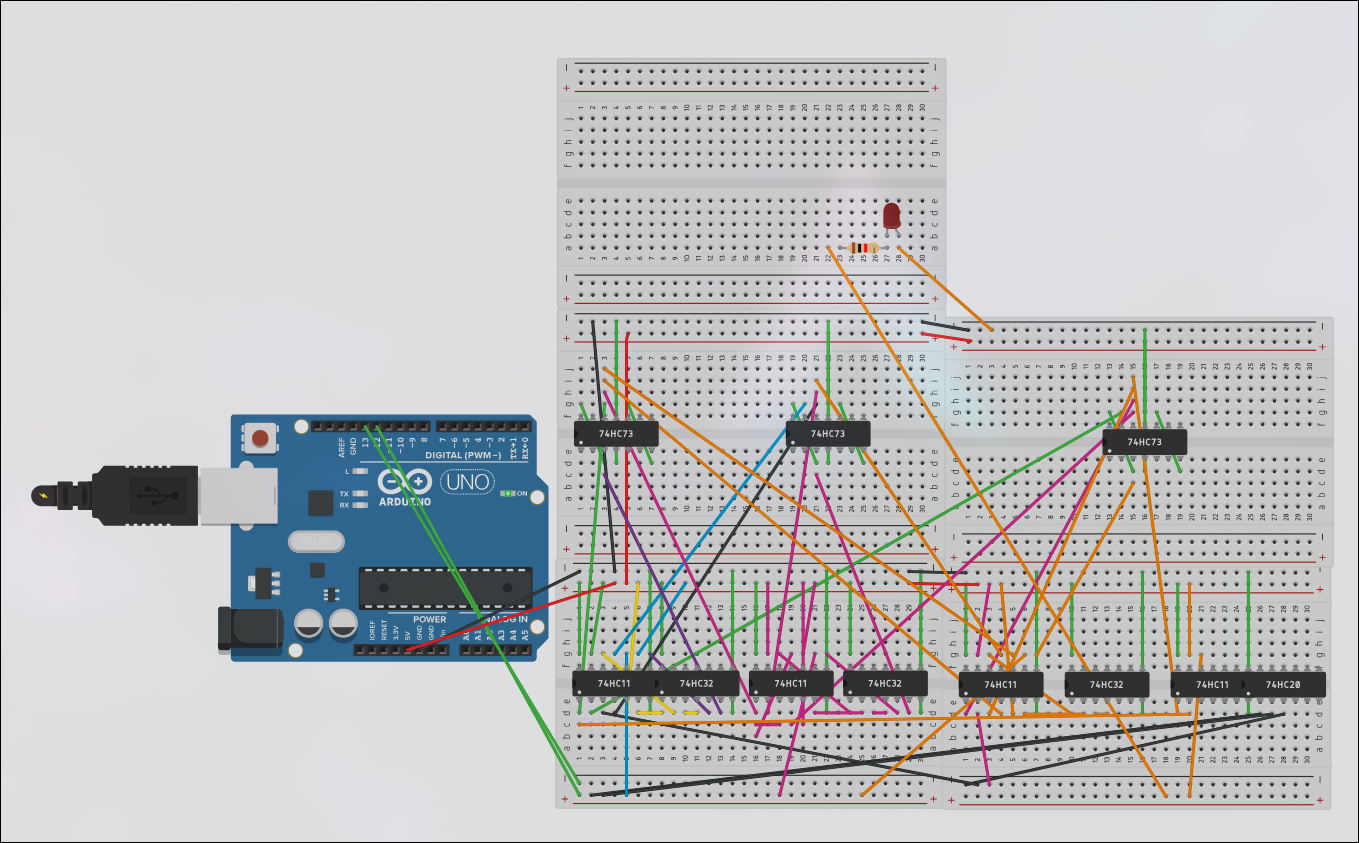
\includegraphics[width=0.8\textwidth]{figs/diagram.png}
    \caption{Circuit Diagram}
    \label{fig:your_image_label}
\end{figure}
\newpage
Below are some schematics for the same,
\begin{figure}[H]
    \centering
    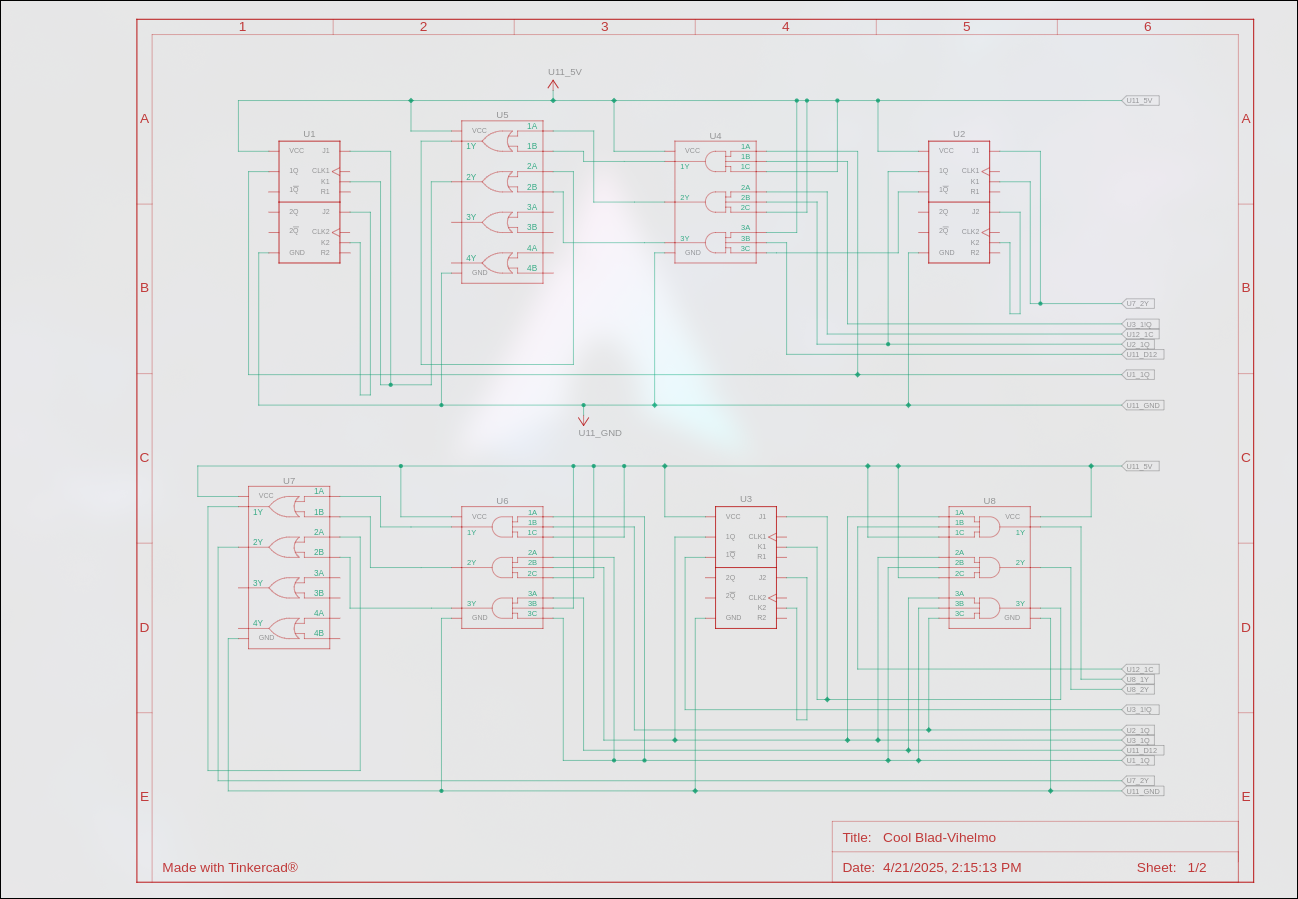
\includegraphics[width=0.8\textwidth]{figs/scheme1.png}
    \caption{Circuit Diagram-01}
    \label{fig:your_image_label}
\end{figure}
\begin{figure}[H]
    \centering
    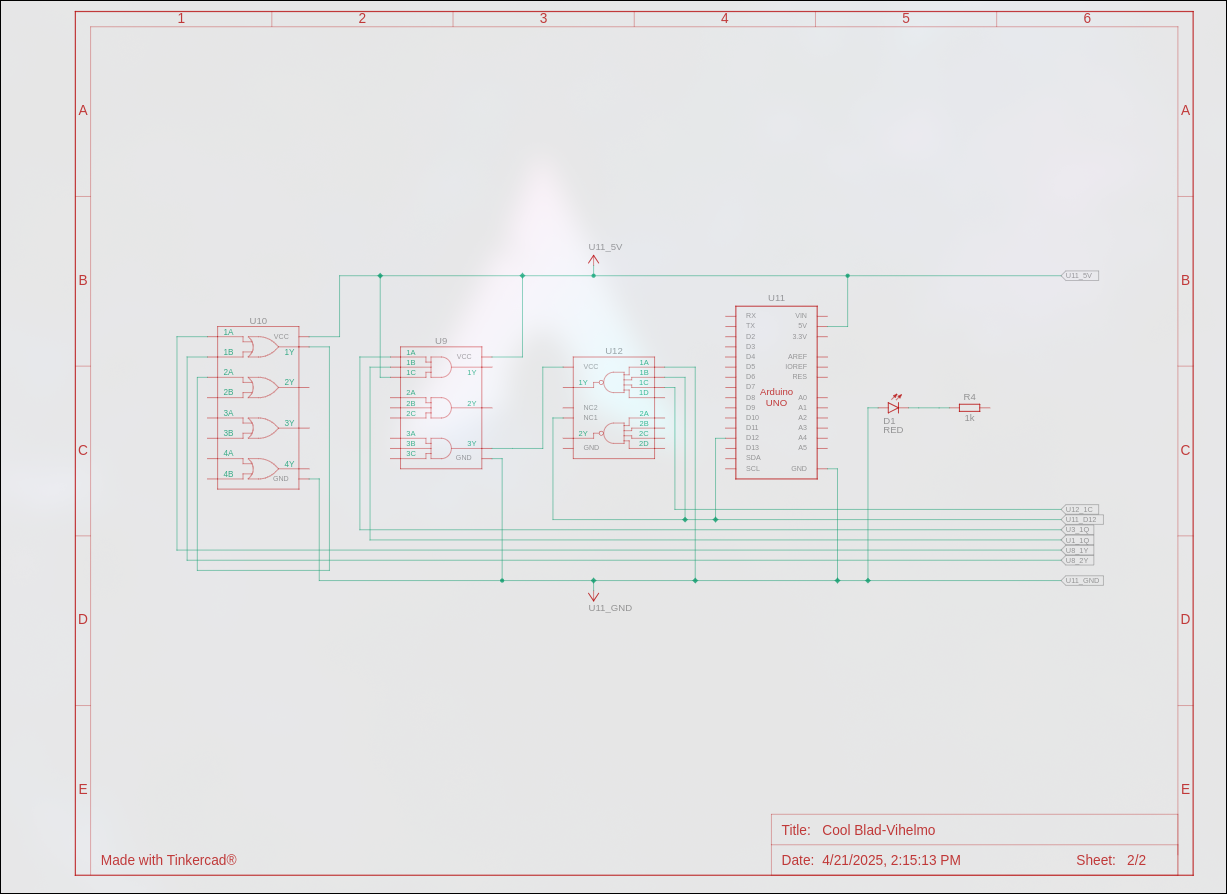
\includegraphics[width=0.8\textwidth]{figs/scheme2.png}
    \caption{Circuit Diagram-02}
    \label{fig:your_image_label}
\end{figure}
\section{Actual Circuit)}
\begin{figure}[H]
    \centering
    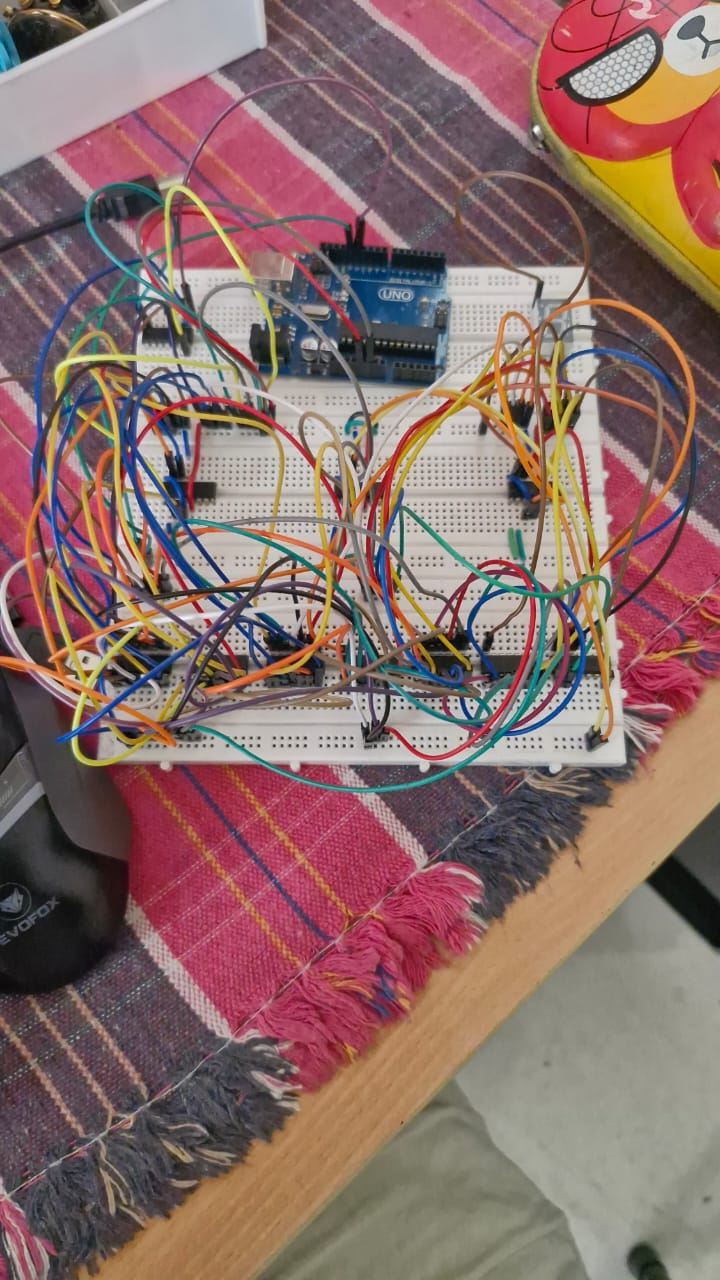
\includegraphics[width=0.8\textwidth]{figs/fig.png}
    \caption{Final Circuit}
    \label{fig:your_image_label}
\end{figure}
\section{The input output wave forms}
\begin{figure}[H]
    \centering
    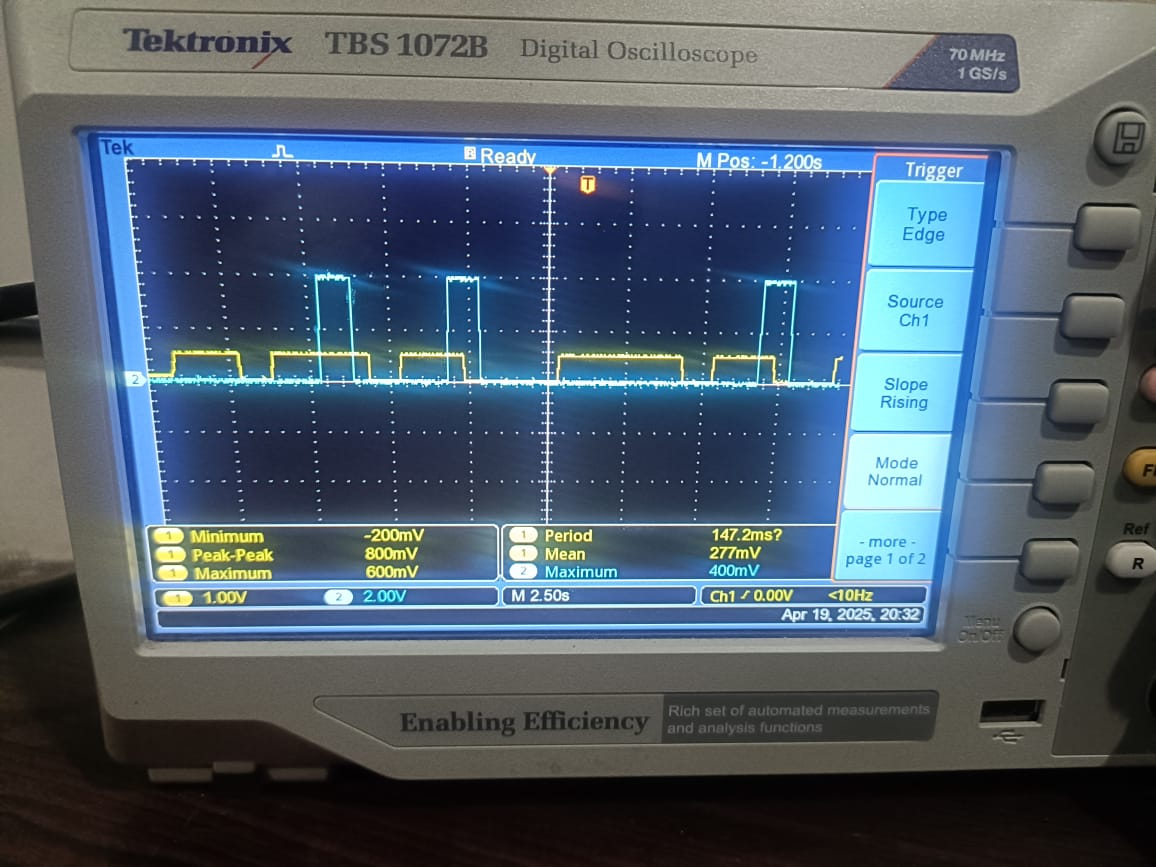
\includegraphics[width=0.8\textwidth]{figs/plot.jpeg}
    \caption{The wave form}
    \label{fig:your_image_label}
\end{figure}

This circuit is designed to detect the sequence 11011 ; orange in colour , overlappingly, which it successfully does . This is clear from the above waveforms , also as expected the output waveform for 11011 goes as 00001, which is also as expectedly shown in the waveform coloured blue

\end{document}

